
\chapter{Exodus}

\section{Introduction}
\label{sec:introduction}

Managing enterprise networks is notoriously challenging~\cite{
benson09unraveling,Casado07Ethane, casado06sane, kim11evolution,sung11systematic,
  yu11vpn}. 
Software-defined networking (SDN) holds the
promise of making this problem easier by centralizing configuration
and management, thereby easing the
evolvability of the network, and enabling the use of novel programming
languages and verification techniques.

However, migrating from an existing, working network environment to
an SDN presents a formidable hurdle~\cite{jain++:sigcomm13-google-sdn}.
Enterprises and administrators are familiar
with, and quite likely depend upon, the specific behavior of existing
configurations, and any SDN replacement will need to begin with identical
behavior.

Unfortunately, these networks can be large 
and complex~\cite{kim11evolution,levin13panopticonTR,zeng12test}, with network behavior
defined by myriad policies, 
%both explicit and implicit, 
usually specified for each individual device, in a variety of
languages that configure distributed programs embedded in these
devices. 
The scale and complexity of the aggregate
behavior of these rules means the process of creating a
controller program for an equivalent SDN is non-trivial.
For example, Purdue's network was reported to
have over 15,000 hosts, 200 routers, 1,300 switches, and 182
VLANs in 2011~\cite{sung11systematic}. 
%
Stanford's backbone, whose publicly available configuration we use in
our evaluation~\cite{zeng12test}, has two
large border routers connected through 10 switches to 14 Operational Zone
routers. In aggregate, the configuration comprises 757,000 forwarding entries
and 1,500 ACL rules. 


Today, there are a few options for incrementally migrating a physical
network to an SDN~\cite{Casado07Ethane, Casado:hotsdn2012-fabric, levin13panopticonTR}, 
which we review later in the paper. However, a common deficiency
of these migration paths is the need to rewrite network policies
and configurations from scratch, a tall order for busy network operators~\cite{Barrett04fieldstudies}.
For a risk-averse network administrator,
this may be reason enough not to migrate. 


%However, few of the world's enterprises are currently using
%SDNs. Instead, most network behavior is defined by the concurrent
%execution of distributed programs running on distinct devices; these
%programs are written in a variety of vendor-specific special-purpose
%languages. Because enterprises and administrators are familiar
%with, and quite likely depend upon, the specific behavior of these
%programs, any SDN replacement will need to begin with identical
%behavior. Unfortunately, 
%In~\cite{levin13panopticonTR} the authors
%evaluate their design on a local campus network comprising 1713 L2 and L3
%switches. Finally, in~\cite{kim11evolution}, the authors report that the
%Georgia Tech and Wisconsin campuses comprise respectively 1097 and 1624
%routers, firewalls, and switches. 

%
This paper directly addresses the problem of migrating distributed network
configurations to equivalent SDN controller programs, and presents Exodus, a
system for performing this conversion. Exodus consumes configurations written
in languages such as Cisco IOS and Linux iptables, and generates programs written in Flowlog, a research
language for SDN programming~\cite{ngdfk:hotsdn13-flowlog}.  Flowlog
provides a compiler and run-time system for controlling OpenFlow switches;
atop this, Exodus generates both the controller software and the switch
configurations needed to execute these programs.  
%It also provides support to
%test the resulting configuration in Mininet~\cite{lantz++:hotnets10-mininet}.
Two of Flowlog's advantages are that it provides rich verification tools (which are not the
focus of this paper), and enables Exodus to generate code we believe is easy to
later evolve and maintain (\Cref{sec:evaluation}).
We will discuss the choice of Flowlog in more detail in \Cref{sec:target}. 

By bootstrapping an SDN controller program with equivalent behavior to
the original network (in full or in part), Exodus's approach lets network
operators iteratively obtain the benefits of centralization.  
For example, Exodus can convert the configuration of just a single router, 
replacing one piece of the network, or it can convert the network's complete
set of configurations. The resulting SDN controller can then be used
to control OpenFlow-enabled switches in the production network,
or it can be used to evaluate the new configuration in a laboratory or
emulation environment.

This automated (and quick!, see \Cref{sec:evaluation}) process gives the network operators time to become
comfortable with their new SDN, before upgrading more critical
components of the network. (For instance, Panopticon~\cite{levin13panopticonTR} shows how
to achieve many benefits of SDN in a cost-aware manner, by only selecting
a few routers at a time for conversion to an SDN; however, Panopticon
does not explain what software to actually \emph{run} on the
controller, the gap that Exodus fills. We discuss alternate approaches to
SDN migration, such as hybrid mode switches, in \Cref{sec:relwork}.)  Only
after the existing policy is successfully migrated may it make sense
to begin reaping additional benefits which are exclusive to SDNs, such
as treating the network as a single ``big switch.''

In keeping with the heterogeneity of modern networks,
Exodus is not limited to IOS. Because it uses a rich intermediate
language based on first-order logic, it can handle other configuration
languages as well, limited only by parsing and translation into this
logic; we have built a translator for Linux iptables as well, and
support features similar to those in Juniper Network's JunOS. Because
the intermediate language is similar enough to Flowlog, we present
only the latter, which is also the concrete output of Exodus. Also, to
make the paper more broadly accessible, we present the compiler
through examples rather than formal rules.

The rest of this paper proceeds as follows: we start by exploring an
input language to our compiler, Cisco IOS, and introduce a running
example program (\Cref{s:bg:ios}).  Next, we describe our chosen
target language, Flowlog, and justify our choice
(\Cref{sec:target}). This is followed by a description
of our system (\Cref{sec:translating}), which we
evaluate on the configurations of a large campus network
(\Cref{sec:evaluation}).  Conducting this research has identified
several interesting weaknesses in current technology, which we discuss
in \Cref{sec:tradeoffs}. We then explain how we can extend our
prototype to cover more features (\Cref{sec:road-ahead}), discuss
related work (\Cref{sec:relwork}), and conclude.

%%%%%%%%%%%%%%%%%%%%%%%%%%%%%%%%%%%%%%%%%%%%%%%%%
\section{Background: Cisco IOS}
\label{s:bg:ios}

We begin by introducing the source language, IOS. IOS is expressive:
it provides not just a ``routing'' language or a ``firewall'' language, but
also a rather wide array of features that we discuss
below. This set of features ensures that our compilation
task is a non-trivial one. (Later in this section, 
we discuss configuration languages other than IOS.)

As a running example for the paper, we present a small enterprise's
configuration, consisting of a pair of networking devices connected as
shown in \autoref{fig:orig-network}. The figure represents two
devices, \ios{int} and \ios{ext}, that sandwich a DMZ. The enterprise
places publicly visible servers, such as the Web server, in this
DMZ. External traffic is allowed to connect to specified servers and
ports in the DMZ, but traffic cannot penetrate further to enter the
corporate LAN. In turn, limited traffic from the corporate LAN is
allowed to egress to the external network. Finally, the external
network is allowed certain carefully delineated
connections with the corporate LAN, as we discuss below.

% Not using Cref here because it isn't recognizing the lst: labels
Listing~\ref{lst:initial-example-int} shows a small IOS configuration for a single
device above. (We will use excerpts from this listing throughout this paper.)
Line 1 defines the name of the router to be \ios{int} (short for
``internal''). Lines 3-5 define an interface (or ``port'') called \ios{in\_dmz},
assign it an IP address and subnet (\ios{10.1.1.1/24}), and indicate
that the router should apply NAT functionality to traffic arriving at this interface
(which is an \emph{outside}, or public-facing, interface). Lines 7-10 define the internal
interface \ios{in_lan}, and assign an ingress filter (via \ios{access-group}) as
well as an IP address and subnet (\ios{192.168.1.1/16}). NAT is enabled here
as well, but as an \emph{inside} interface.

Lines 12-15 define the access-list (or ACL) \ios{102}, which is used to filter traffic
arriving at \ios{in_lan}. It says that: \ios{ip} packets arriving from \ios{192.168.4.1/24}
should be denied access to the \ios{10.1.1.3} host, \ios{tcp}
packets from any source destined for \ios{10.1.1.3:25} are permitted, as are
\ios{tcp} packets to port \ios{80} on any host. Other packets are denied. IOS
resolves conflicts between these rules using the standard first-applicable
semantics: A packet from the forbidden subnet will be denied, even if it is
destined for \ios{10.1.1.3:25}.

\begin{figure}
  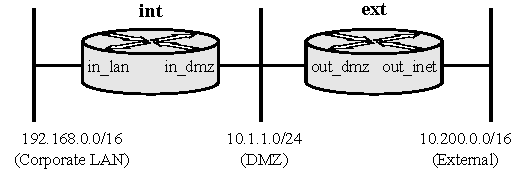
\includegraphics[scale=0.95]{figs/orig_network.pdf}
  \caption{Topology for Example Network}
  \label{fig:orig-network}
  \hrule
\end{figure}

Line 17 configures NAT for the router. In this case, all outgoing packets will
be rewritten to have source address \ios{10.1.1.1} (\ios{interface in_dmz}).
The \ios{overload} keyword enables multiple internal devices to map to the single
external address, multiplexing via the traditional Layer-4 attributes. While IOS also
allows a pool of external addresses to be used, that feature is beyond the
scope of this example. Access-list \ios{1} dictates which packets NAT should
apply to. Line 18 defines access-list \ios{1}, which matches all packets from
the subnet on \ios{in_lan}. Finally, line 20 introduces a default route.
If a packet is destined for an address outside the two interfaces'
subnets, \ios{10.1.1.2} will be its next-hop router.

\Cref{lst:initial-example-ext} provides the configuration for the
other device, \ios{ext}. The IOS features it uses are mostly identical
to those in \Cref{lst:initial-example-int}. This router
shares the DMZ subnet ({\small\verb$10.1.1.0/24$}) with the
\ios{int} router. Its other interface exits the example network via subnet
\ios{10.200.0.0/16}. The one major difference is that this device uses
a \emph{reflexive} access-list.

% This is our home-grown India talk example, NOT a forum post.
\noindent\begin{minipage}{\linewidth}
\begin{lstlisting}[float=t,label=lst:initial-example-int,language=IOS,caption=Example IOS Configuration (1)]
hostname int

interface in_dmz
ip address 10.1.1.1 255.255.255.0
ip nat outside

interface in_lan
ip access-group 102 in
ip address 192.168.1.1 255.255.0.0
ip nat inside

access-list 102 deny ip 192.168.4.1 0.0.0.255 host 10.1.1.3
access-list 102 permit tcp any host 10.1.1.3 eq 25
access-list 102 permit tcp any any eq 80
access-list 102 deny any

ip nat inside source list 1 interface in_dmz overload
access-list 1 permit 192.168.1.1 0.0.255.255

ip route 0.0.0.0 0.0.0.0 10.1.1.2
\end{lstlisting}
\end{minipage}

\noindent\begin{minipage}{\linewidth}
\begin{lstlisting}[float=t,label=lst:initial-example-ext,language=IOS,caption=Example IOS Configuration (2)]
hostname ext

interface out_dmz
ip access-group 103 in
ip address 10.1.1.2 255.255.255.0

interface out_inet
ip access-group 104 in
ip address 10.200.1.1 255.255.0.0

ip access-list extended 103
  deny ip any host 10.200.200.200
  deny tcp any any eq 23
  permit tcp host 10.1.1.1 any eq 80 reflect returnflow
  permit tcp host 10.1.1.1 any eq 22 reflect returnflow
  deny any

ip access-list extended 104
  deny 10.200.200.200
  permit tcp any host 10.1.1.3 eq 25
  permit tcp any host 10.1.1.4 eq 80
  evaluate returnflow
  deny any
\end{lstlisting}
\end{minipage}

Reflexive access lists are used to dynamically open temporary
firewall holes to permit return packets for approved outgoing flows.
The rules on lines 14-15 allow outgoing
web and SSH traffic from the NAT address, with the additional stipulation \ios{reflect returnflow},
which creates a table (and gives it the name \ios{returnflow}) of ongoing
flows approved by this rule. Line 22 evaluates this table, permitting the return
traffic. Note the lack of a \ios{permit tcp any host 10.1.1.1} rule to permit the NAT's return traffic; such a
rule is both overly broad and unnecessary due to the reflexive ACL configuration.


\paragraph{Other Configuration Languages}

So far, we have discussed only the IOS language. Our parser also
handles a significant subset of the Linux iptables language, which has
similar functionality but different syntax. For instance, consider the
following configuration (which mirrors the permit rule on line 13 of \Cref{lst:initial-example-int}):

\begin{lstlisting}[label=lst:iptables,language=IOS]
iptables -A INPUT -i int_lan 
         -d 10.1.1.3 -dport 25 
         -p tcp -j ACCEPT
\end{lstlisting}

\noindent
Exodus has an internal, logic-based intermediate language that serves
as a target of all these compilers. Because this intermediate language
is agnostic to surface syntax, we believe Exodus can also work
well with other popular (and in some cases, competing) configuration
languages, such as Juniper's JunOS. Nevertheless, for simplicity, the
rest of this paper is written in terms of IOS.

\paragraph{Exodus Compiler Coverage: Challenges and Scope}

There are numerous challenges involved in converting such configurations to
SDN. First, the text to be converted describes multiple small programs: packet
filtering, NAT, static routing tables, and local-subnet routing. Each of these must
be faithfully translated by the compiler. Second, the semantics of these
programs resides in the firmware that interprets them; uttering \ios{ip nat
inside} does not describe how to implement the NAT, but merely configures it
according to the available settings. Third, the configuration is tailored to
a single network appliance; every such device on the network has a separate
configuration that describes its local behavior. A complete translation to SDN must
integrate all such devices into a single, unified system.

Finally, the IOS language is
used in a variety of different network appliances, and exposes many additional
features (e.g., deep packet inspection, dynamic routing, multicast groups,
DoS protection, VPNs, and more) beyond those already presented.
Moreover, even basic features of IOS can exhibit a
sometimes baffling array of variant syntax. For instance, the \ios{access-list}s
of Listing~\ref{lst:initial-example-int} could have been written
differently, as an \ios{ip access-list}, using similar but not identical
syntax as seen in Listing~\ref{lst:initial-example-ext}.

As an initial step, we have focused on an essential set of
features rather than attempting to convert all of IOS. To date, our IOS-to-SDN
compiler supports:
\begin{enumerate}
\item interface and subnet configurations;
\item standard and most extended IOS ACLs, including reflexive access-lists;
\item static routing tables, and policy-based static routing; and
\item ACL-based ``overload'' NAT.
\end{enumerate}
It also accepts multiple IOS configurations to produce a single SDN program.

Overload NAT (an IOS term for port address translation, where a single public
IP address is multiplexed by Layer-4 attributes) was chosen to demonstrate the
viability of our compilation technique; the same techniques could be used to
support other varieties, such as static network address translation, or a NAT
employing a pool of IP addresses. We defer further discussion of how to extend our
compiler to support additional IOS features until~\Cref{sec:road-ahead}.

%TODO: SK comment from train: say ``compiler'', not ``language'' for this community.

%IOS naturally has features for more complex networking operations, such as
%running dynamic routing protocols and deep-packet inspection. Our compiler
%does not currently support these features, but we discuss them as future work
%in \Cref{sec:conclusion}.


\section{Compilation Target}
\label{sec:target}

Since our goal is to translate a collection of IOS policies into an SDN
controller program, we must select a target controller platform. There
are many options: C++ code for the NOX platform~\cite{gude:ccr08-nox},
Python code for POX~\cite{pox}, or Java atop Floodlight~\cite{floodlight}. There are also
numerous research languages
available~\cite{foster:icfp11-frenetic,katta:xldi12-flog,monsanto++:nsdi13-pyretic,ngdfk:hotsdn13-flowlog,Voellmy:2011,voellmy:hotsdn12-procera,Voellmy:2013}.
Our final choice was motivated by the
following needs:
\begin{description}

\item[Output in a High-Level Language] After the policies have been
  turned into SDN programs, they will not remain static: instead, they
  will need to be modified as the network and its requirements
  evolve. Therefore, it is important to produce programs that are not
  so low-level that they end up being regarded as
  ``write-only''. Instead, we must target a meaningfully high-level
  language, and produce relatively readable output in that
  language. This requirement makes the highly expressive research
  languages~\cite{foster:icfp11-frenetic,katta:xldi12-flog,koponen++:nsdi14-vmware-nlog,ngdfk:hotsdn13-flowlog,Voellmy:2013} an attractive choice.

  One advantage to producing high-level code is that it can also then
  be subjected to program analysis and verification activities, which
  will better support evolution of the controller software. There is a
  wide and growing range of such tools, though the most powerful,
  \emph{sound} tools seem to be built for research languages~\cite{guha:sdnverif,ngdfk:hotsdn13-flowlog}.

\item[Support for Controller State] As we have already seen, policies
  refer extensively to state.  The resulting controller programs must
  be able to support NAT, reflexive access lists, and other features
  that dynamically affect how packets are handled.  Thus, the target
  SDN platform must support stateful controller programs, and allow
  the modification of network behavior based on controller state.

  While platforms like NOX obviously support these, some research
  languages do not~\cite{monsanto:popl12-netcore,monsanto++:nsdi13-pyretic,Voellmy:2013}. This requirement also bars us from using
  the simplest of targets -- OpenFlow switch rules -- as they are
  stateless and cannot themselves implement these dynamic policies~\cite{McKeown:ccr08-openflow}.
  High-level languages with built-in state include Maple's algorithmic
  policies~\cite{Voellmy:2013}, and the rule-based languages Nlog~\cite{koponen++:nsdi14-vmware-nlog}, Flog~\cite{katta:xldi12-flog} and Flowlog~\cite{ngdfk:hotsdn13-flowlog}.

\item[Support for Proactive Compilation] Recent
  research has shown how to proactively
  compile high-level SDN programs to OpenFlow flow tables without
  programmer intervention~\cite{monsanto:popl12-netcore}. Selecting such a platform removes the need
  for our compiled SDN programs to micro-manage flow-table updates on
  switches, and allows us to focus on the core goals of this
  project. %More recently, Flowlog has shown how to extend proactive
  %compilation to programs with internal state~\cite{ngdfk:hotsdn13-flowlog}.

\item[Availability as Open Source] Finally, as developing our IOS
  compiler required us to extend the target language in numerous ways
  (\Cref{sec:relwork}), having an open source implementation was
  a necessity. This requirement eliminated several candidate languages
  (e.g., both Maple and Nlog are closed-source).

\end{description}
This collection of requirements induced us to choose Flowlog as
our target language. By doing so, our compiler can generate high-level
rule-based code, and exploit an existing proactive compiler (which in
turn relies on the Frenetic project's
NetCore language~\cite{monsanto:popl12-netcore}) to OpenFlow. In
addition, Flowlog has powerful verification tools to support the
evolution of the generated controller program.

However, we do not claim that the choice of Flowlog is
canonical. Though we have presented arguments in favor of it,
the choice of target language is also a matter of taste:
some might prefer Java or C++ generated for Floodlight or
NOX to programs in a rule-based
language. Nevertheless, Flowlog does provide a stateful,
proactively-compiled language which therefore serves as an excellent
target for compilation; therefore, \emph{we can view Flowlog the
  language as merely an API for its proactive compiler}. The ideas of
this paper apply just as well to other compilation targets, though the
engineering decisions are likely to be rather different (e.g., if one
were generating C++ code that needed to proactively manage OpenFlow
rules).

\paragraph{Flowlog Example}

Since we will use Flowlog to show the output of compilation in the remainder of the
paper, we begin with an illustrative example, which we explain line-by-line:

\begin{lstlisting}[label=lst:flowlog-intro,language=Flowlog]
TABLE seen(ipaddr);
ON ip_packet(pkt):
  DO forward(new) WHERE
    new.locPt != pkt.locPt;
  INSERT (pkt.nwSrc) INTO seen WHERE
    pkt.nwDst IN 10.0.0.0/16 
    AND NOT seen(pkt.nwSrc);
\end{lstlisting}

\noindent
Line 1 declares a one-column table of IP addresses. As tables are a common
representation of network data, used for routing tables, ARP caches, NAT tables,
and more, the Flowlog runtime maintains state in the form of a database.

The remainder of the program comprises two \emph{rules}, both of which are
triggered by any IP packet arrival (line 2) on the network. The first rule (lines 3-4)
implements a basic ``flood'' forwarding policy; the \ios{pkt.locPt} term
represents the incoming packet's arrival port, and the \ios{new.locPt} term
represents the packet's egress port. If multiple valid egress ports exist, the
packet will be sent out of all of them. The second rule (lines 5-7) inserts the
packet's source IP address into the table if the packet is destined for the
\ios{10.0.0.0/16} subnet, and the address is not already stored in the table.

\paragraph{Flowlog Runtime}

The Flowlog runtime is implemented in OCaml, and is built atop the
NetCore and OCaml-OpenFlow packages. Packet arrivals, switch
connections, and other OpenFlow events are passed via NetCore to
Flowlog, where they trigger appropriate rules. For instance, IP
packets would trigger the two rules in the example above.
Correspondingly, changes in Flowlog tables are propagated by its
runtime back to NetCore, which in turn updates OpenFlow rules on the
relevant switches.

Although the program's text makes it appear that every packet is seen by the
program, Flowlog's proactive compiler is in fact far more efficient. The
switch rules it produces ensure that the only packets that reach the controller are ones that will
change its internal state (in this example, packets with
as-yet-unseen source addresses).

% Naw, don't bother ... this isn't a NetCore paper. these are easy to understand.
%{\color{blue}
%[ADF: The NetCore samples which follow are excellent. Should we also include
%the OpenFlow rules? perhaps in an appendix? Remember, our reviewers are not
%expected to have seen Flowlog before this.]}


When we execute the above Flowlog program, it compiles into the following
initial NetCore policy, which is then distributed to the switches by the NetCore runtime:
\begin{lstlisting}[label=lst:flowlog-netcore-1,language=Flowlog]
(filter dlTyp = ip; all) +
(filter dlTyp = ip &&
        dstIP = 10.0.0.0/16; fwd(OFPP_CONTROLLER))
\end{lstlisting} 
Line 1 specifies that all \ios{ip} packets be flooded. Line 2 selects the packets
of interest and sends them to the controller.
If \ios{10.0.0.1} pings \ios{10.0.0.2}, the controller receives
both the initial echo request and reply packets. It adds both IP addresses to its state
table, and issues a new policy that ensures it does not see packets from those
hosts again:
\begin{lstlisting}[label=lst:flowlog-netcore-2,language=Flowlog]
(filter dlTyp = ip; all) +
(filter (dlTyp = ip && 
         dstIP = 10.0.0.0/16) &&
         !(srcIP = 10.0.0.1 ||
            srcIP = 10.0.0.2);
 fwd(OFPP_CONTROLLER))
\end{lstlisting}

%%%%%%%%%%%%%%%%%%%%%%%%%%%%%%%%%%%%%%%%%%%%%%%%%
\section{From IOS to SDN}
\label{sec:translating}

\begin{figure}
  \centering
  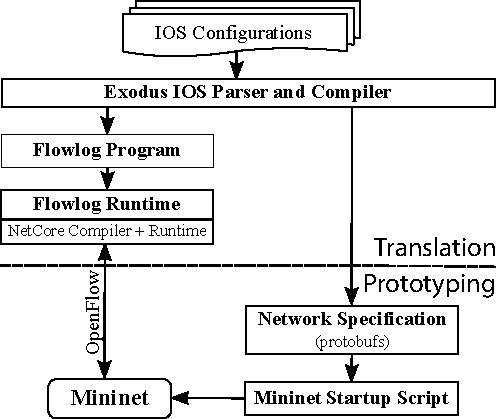
\includegraphics[scale=0.9]{figs/workflow.pdf}
  \vspace{0.2cm}
  \caption{Exodus Workflow}
  \label{fig:workflow}
  \hrule
\end{figure}

Now we present our core technical contribution. Our goal is the
workflow of \Cref{fig:workflow}. For instance, given the examples from 
\Cref{lst:initial-example-int} and \Cref{lst:initial-example-ext}
stored as files \fl{natfw.txt} and \fl{outerfw.txt} respectively, the
user runs:

{\centering \fl{\ \ exodus natfw.txt outerfw.txt}}

\noindent
This produces an SDN system that mirrors the network behavior
represented by these IOS configurations. Given this two-device
configuration, Exodus produces an SDN system for two OpenFlow switches
wired in the same way, each holding six tables. It also
produces Flowlog code that uses these OpenFlow tables, together with
internal state relations, to reproduce the behavior of the original
devices.

We present this process in three steps. First (\Cref{sec:net-conf}), we
describe the flow tables, and explain how we map them to
current OpenFlow hardware. Second (\Cref{sec:code-gen}), we describe
the compiler from IOS to Flowlog that generates the controller
software. Finally (\Cref{sec:prototyping}), we discuss
deploying and running the resulting system using the
complete Exodus tool suite, which is publicly available on Github.

\subsection{Network Configuration}
\label{sec:net-conf}

Exodus needs to reflect the semantics of IOS and the requirements for
IP routers (RFC 1812~\cite{rfc1812}). To do so, Exodus creates six logical
OpenFlow tables per router in the original configuration: two for access-control, two for routing, and one each
for Layer-2 rewriting and NAT, as shown in \autoref{fig:flowlog-router}(a).
These tables cannot actually implement these features;
that requires support from the controller. Rather, they implement the
corresponding stage of the processing pipeline,
dropping, rewriting, or forwarding packets as dictated by the controller.

The sequential composition of tables in \autoref{fig:flowlog-router}(a)
maps to OpenFlow 1.1+'s pipeline of multiple tables, and echoes the
hardware pipelines of traditional, non-OpenFlow routers.  Packets
first enter from the subnets on the left, where an inbound ACL is
applied before forwarding them to the second stage, which implements
the routing table.  The routing table also determines if a packet
needs to be translated. If so, if goes through the NAT table, and then
through a second round of routing. The fifth stage sets the
destination MAC address. A final access check is performed in the
outbound ACL table, before the packet reaches the intended subnet.

In OpenFlow 1.0, which we use due to its mature support, sequential composition
is well-known to create large numbers of rules due to the necessary
cross-products.  To keep the number of rules in check, Exodus \emph{physically}
performs the composition by wiring four single-table switches in series (see
\autoref{fig:flowlog-router}(b)).
Our current pipeline is designed to minimize the number of switches; we
``fold'' the tables in a symmetric arrangement around the NAT, and packets flow
in both directions. In the inbound direction, the second table, L2 Rewrite, is
just a pass-through.

Our design prepares Exodus for transition to newer versions of OpenFlow with
support for multiple tables.  It also makes clear the features needed by each
flow table, allowing one to program a single switch with the
protocol-independent packet processors proposed
in~\cite{Bosshart:2013ppipp-arxiv}: the ACL tables may match any field, but
only need to drop or forward packets; the routing table forwards packets based
on masked IP addresses; the NAT table performs Layer-3 rewriting and exact
matching; and the Layer-2 rewriting has many ``narrow'' entries, matching on IP
addresses and setting the corresponding MAC addresses of all connected hosts.

\begin{figure}
  \centering
  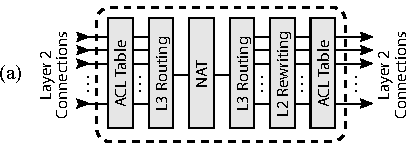
\includegraphics[scale=0.9]{figs/flowlog-router-unfolded}
  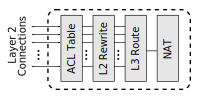
\includegraphics[scale=0.9]{figs/flowlog-router-folded}
  \caption{Logical flow tables in an Exodus router implementation (a), and the implementation
with physical switches in OpenFlow 1.0 (b).}
  \label{fig:flowlog-router}
\end{figure}

Of the four types of flow tables used by Exodus, three -- ACL, routing,
and NAT -- are managed by code generated from the IOS configuration (as
described in \Cref{sec:code-gen}). The fourth, Layer-2 rewriting,
is independent of IOS, and simply sets the destination MAC address
on outgoing, routed traffic. To populate this, we developed an
ARP Proxy, which allows the router to respond to ARP requests
for its interfaces and known hosts, and to issue queries on the attached
subnets.

\subsection{Code Generation}
\label{sec:code-gen}

The heart of Exodus is a compiler that converts IOS into Flowlog that
runs on the controller.  We present the compiler by describing its
treatment of each supported feature.  Separately, we have modified
Flowlog's proactive compiler so actions generated by each of
these features are mapped to the OpenFlow switch tables
corresponding to that feature.

\subsubsection{Static and Policy-Based Layer-3 Routing}

The core purpose of a router is Layer-3 routing.
The Exodus compiler translates IOS routing tables into Flowlog code
that manages the OpenFlow tables responsible for routing. For instance,
consider the default route given on line 20 of \Cref{lst:initial-example-int}.
Each such rule is compiled into a Flowlog fragment that defines a next-hop IP
address for incoming packets. In this case, only a ``default'' route
needs to be specified for all packets arriving at the \ios{int}
router:
\begin{lstlisting}[label=lst:routing-flowlog,language=Flowlog]
routerAlias("int", pkt.locSw) 
  AND (10.1.1.2 = nexthop)
\end{lstlisting}

\noindent
\fl{routerAlias} is an empty Flowlog relation defined by Exodus and
populated by code generated by the compiler. It maps between the
string-based names in IOS and the numeric identifiers in
OpenFlow. The fragment assigns a value (\fl{10.1.1.2}) to the next-hop
for all packets arriving at the \fl{int} router; the value is then
used by the modified Flowlog compiler to populate the appropriate
OpenFlow table.

Exodus's output also assigns next-hops based on IOS's ``policy
routing'' feature, which assigns next-hops to packets
based on access-lists. While our main example does not
use this feature, an interface might be configured as:

\begin{lstlisting}[label=lst:policy-route-decl,language=IOS]
hostname example
interface eth0
ip policy route-map internet
\end{lstlisting}

\noindent Line 3 specifies that the policy named \ios{internet} should
be applied to traffic on this interface. The \ios{internet} policy
must be defined in the configuration, as in the following example
(from \cite{n++:lisa-margrave-firewalls}):

\noindent\begin{minipage}{\linewidth}
\begin{lstlisting}[label=lst:policy-route,language=IOS]
access-list 10 permit 10.232.0.0 0.0.3.255

route-map internet permit 10
match ip address 10
set ip next-hop 10.232.0.15
\end{lstlisting}
\end{minipage}

\noindent
Line 1 of the policy defines a set of packets to apply a next-hop
address to. Lines 3-5 specify that address -- in this case,
\ios{10.232.0.15}.  As in the static-routing case, Exodus creates a
corresponding Flowlog fragment that assigns the appropriate next-hop
for matching packets:
\begin{lstlisting}[label=lst:policy-routing-flowlog,language=Flowlog]
routerAlias("example", pkt.locSw)
  AND portAlias("example", "eth0",
    pkt.locPt) 
  AND pkt.nwSrc IN 10.232.0.0/22
  AND 10.232.0.15 = nexthop
\end{lstlisting}

\noindent Line 1 filters on the packet's switch location. Lines 2-3
match the interface the packet arrived from;
\fl{portAlias} is another Flowlog relation that maps between the
string-based interface names in IOS and OpenFlow's numeric port
identifiers. Line 4 applies the access-list, making certain that only
packets from \ios{10.232.0.0/22} receive the next-hop address given
by line 5. As in the static-routing case, the next-hop value is then
used by the modified Flowlog compiler to produce OpenFlow switch
tables.

\subsubsection{Packet Filtering}
\label{sec:filtering}

We now turn to the OpenFlow tables for ingress and egress ACLs.
Consider the rules on lines 12-13 of \Cref{lst:initial-example-int}.
This ACL can be trivially represented as OpenFlow rules of essentially the
same form, using the ``drop'' action for the \ios{deny} rule, and forwarding
otherwise. As
Flowlog currently uses negation in place of an explicit ``drop'', the compiler
embeds \ios{deny} rules as negative conditions; e.g. lines 3-4 of:
\begin{minipage}{\linewidth}
\begin{lstlisting}[label=lst:flowlog-filter,language=Flowlog]
ON tcp_packet(pkt): 
  DO forward(new) WHERE
    NOT (pkt.nwSrc IN 192.168.4.1/24
      AND pkt.nwDst = 10.1.1.3)
    AND pkt.nwDst = 10.1.1.3 
    AND pkt.tpDst = 25
\end{lstlisting}
\end{minipage}

\noindent
As IOS allows an interface to have separate ingress and egress
filters, Exodus produces separate Flowlog fragments for
each. This does not add any notable complexity to the output, and is
in keeping with the router pipeline described in \Cref{sec:net-conf}.

\subsubsection{Reflexive ACLs}

Whereas ordinary ACLs required no controller state, reflexive
access-lists do. A rule tagged with \ios{reflect}, like those seen on
lines 14-15 of \Cref{lst:initial-example-ext}, matches traffic like a
normal ACL rule, but also causes the device to remember the traffic's
source and destination for later use. A corresponding \ios{evaluate}
rule, like the one on line 22 of the same configuration, uses that
memory to permit return traffic.

While static ACLs can explicitly permit return traffic, dynamically adding new
such rules requires the SDN controller. Thus, in an SDN
context, reflexive access-lists must be managed by the controller, as we describe next,
rather than performed entirely by the switch.

\paragraph{Stage 1: ``Reflect'': Remembering Outgoing Traffic}

To hold the state on the controller, Exodus uses a
relation called \fl{reflexiveACL}, which contains a row for each
hole to be opened in the firewall. This state relation 
resides on the \emph{controller}, and Flowlog's runtime will use it to
automatically keep the ACL tables on the switches up to date. To declare
the new state relation, the compiler generates:

\begin{lstlisting}[label=lst:flowlog-racl-table,language=Flowlog]
TABLE reflexiveACL(string, ipaddr, 
  tpport, nwproto, ipaddr, tpport);
\end{lstlisting}

Column 1 of this relation stores the identifier (in this case, \ios{returnflow})
used for the traffic of interest. Columns 2-6 store the standard
flow-identification information. For every matching \ios{reflect} in the IOS
ACL, the compiler creates a corresponding Flowlog \fl{INSERT}
rule. For instance, the rule on line 14 compiles into:

\begin{lstlisting}[label=lst:flowlog-racl-insert,language=Flowlog]
ON tcp_packet(pkt):
  INSERT ("returnflow", pkt.nwSrc, 
    pkt.tpSrc, pkt.nwProto, pkt.nwDst,
    pkt.tpDst) INTO reflexiveACL
  WHERE pkt.nwSrc=10.1.1.1 
  AND pkt.tpDst=80
  AND aclAlias("ext-out_dmz-acl", 
    pkt.locSw, pkt.locPt, ANY) 
  AND NOT reflexiveACL("returnflow", 
    pkt.nwSrc, pkt.tpSrc, pkt.nwProto, 
    pkt.nwDst, pkt.tpDst);
\end{lstlisting}
Lines 5-6 ensure that the ACL rule actually applies to the packet in
question, and lines 7-8 enforce that the check applies only to the
proper router and interface names. 

\paragraph{Stage 2: ``Evaluate'': Permitting Return Traffic}

For every \ios{evaluate} clause in the original configuration, the compiler asserts a
corresponding ACL rule in Flowlog. These rules resemble those of \Cref{sec:filtering},
and also refer to the \fl{reflexiveACL} state table:

\noindent % needed to prevent indentation of entire code block
\begin{minipage}{\linewidth}
\begin{lstlisting}[label=lst:flowlog-racl-rule,language=Flowlog]
  aclAlias("ext-out_inet-acl", pkt.locSw, 
    pkt.locPt, new.locPt)  
  AND reflexiveACL("returnflow", 
    pkt.nwDst, pkt.tpDst, pkt.nwProto, 
    pkt.nwSrc, pkt.tpSrc) 
  AND (22 = pkt.tpSrc) 
  AND (10.1.1.1 = pkt.nwDst) AND 
  NOT (10.200.200.200 = pkt.nwsrc)
\end{lstlisting}
\end{minipage}

\noindent
This example encodes the \ios{evaluate} rule on line 22 of
\Cref{lst:initial-example-ext}. The \fl{aclAlias} reference
limits the rule to the proper router and interface. The
reference to the \fl{reflexiveACL} table on lines 3-5 has a reversed
ordering from the above \fl{INSERT} rule;
this is because the insertion rule triggered on outgoing traffic, while
this rule filters incoming traffic for the same flow. The final line
prevents the rule from applying if the higher priority deny rule
(line 19 of \Cref{lst:initial-example-ext}) would.

\subsubsection{Network Address Translation}

NAT presents two challenges. First, like reflexive access-lists, NAT
in SDNs requires some amount of controller management; Exodus must
produce Flowlog code that governs the dynamic nature of NAT. Second, NAT
\emph{changes} the headers of packets as they are forwarded. While
header-mutation is a primitive action in OpenFlow, the exact values
used depend on the NAT's overall state.

As mentioned in \Cref{s:bg:ios}, our compiler currently supports only one of
the many types of NAT available in IOS: dynamic port-address translation using
a single public IP. This is sufficient to show the feasibility of our
approach; static NAT is simpler as it requires no controller state,
and pool NAT only requires an additional table of available public IPs.

The compiler produces Flowlog code that, on controller start, populates
state relations describing how NAT should be performed. For example,
these values for \Cref{lst:initial-example-int}:
\begin{lstlisting}[label=lst:flowlog-nat-startup,language=Flowlog]
ON startup(e):
  INSERT (0x100000000001, 192.168.0.0, 16) 
    INTO needs_nat;
  INSERT (0x400000000001,1,1,10.1.1.1) 
    INTO natconfig;
  INSERT (10.1.1.1, 0x6, 10000) 
    INTO seqpt; 
  INSERT (10.1.1.1, 0x11, 10000) 
    INTO seqpt; 
\end{lstlisting}

\noindent
Line 1 states that the insertions happen at controller
startup. Lines 2-3 record that new flows from the private IP
\ios{192.168.0.0/16} must be subject to NAT on a given switch. Lines 4-5 configure a
related switch to use the given external IP address for this
translation. Lines 6-9 set up initial port values for NAT (port
\ios{10000} for both TCP and UDP).

Exodus also includes a library, a fragment of which is shown below, that
contains rules that utilize these
tables. These describe, for instance, how to handle new TCP traffic from the
internal subnet:

\noindent % needed to prevent indentation of entire code block
\begin{minipage}{\linewidth}
\begin{lstlisting}[label=lst:flowlog-nat-port-assign,language=Flowlog]
ON tcp_packet(pkt) WHERE 
  NOT ptassign(0x6, pkt.nwSrc, pkt.tpSrc, 
    ANY, ANY)
  AND natconfig(pkt.locSw, pkt.locPt,
    publicLocPt, publicIP) 
  AND NOT natconfig(pkt.locSw, ANY, 
    ANY, pkt.nwDst) 
  AND seqpt(publicIP, 0x6, x) 
  AND add(x, 1, publicPt):
  INSERT (0x6, pkt.nwSrc, pkt.tpSrc,
    publicIP, publicPt) INTO ptassign;
  DO forward(new) WHERE
    new.locPt = publicLocPt 
    AND new.nwSrc = publicIP 
    AND new.tpSrc = publicPt
    TIMEOUT 600;
\end{lstlisting}
\end{minipage}

\noindent
Lines 2-3 dictates that no NAT port has yet been assigned to this
flow. Lines 4-5 extracts the public IP address to be used. Lines 6-7
prevents the rule from applying if the packet is being sent to a
public IP that is reserved for NAT (i.e., if it is return
traffic). Lines 8-9 produce a fresh TCP port by incrementing the one used most recently. Lines 10-11 record the port
used and the source of the NAT flow (for translating future packets in
the flow). Lines 12-16 send this initial packet on its way; the final
\fl{TIMEOUT} line applies a 600-second idle timeout to the forwarding
rules, which allows the program to reclaim expired NAT ports for later
use.

Although the tables and the data here are different, this process is similar
to how the compiler handles reflexive access-lists. While space restrictions prevent us
from giving the entire NAT program, the rules produced for return traffic, UDP
traffic, etc.\ are similar.

\subsection{Prototyping the Network}
\label{sec:prototyping}

\begin{figure}
  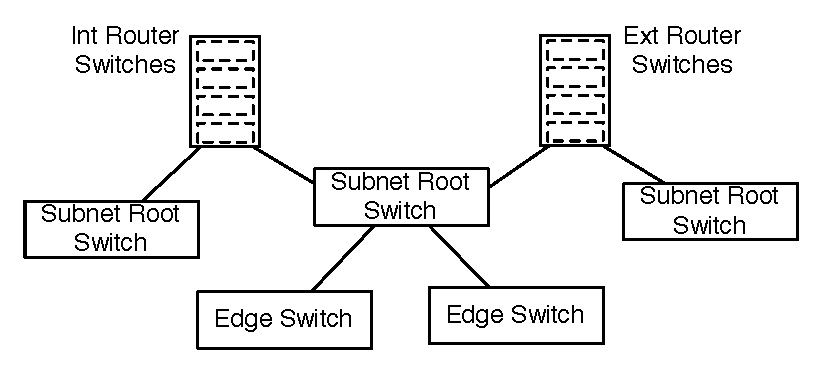
\includegraphics[width=0.45\textwidth]{figs/flowlog-network.pdf}
  \caption{Two Exodus routers attached to a shared subnet}
  \label{fig:flowlog-network}
\end{figure}

Exodus produces more than just a Flowlog program: it also produces a
description of the network on which it runs, including the switches, their
wiring, and configuration, which allows us to have a running prototype of the
network in an emulation environment such as Mininet~\cite{lantz++:hotnets10-mininet}. The specification can also
serve as a blueprint for a physical network that implements the same policies
as the original network.

These configuration values are loaded into the Flowlog program on startup,
which then interacts with the corresponding tables in the physical or
emulated network.  The compiler outputs the complete description in a custom
Google Protocol Buffers format~\cite{protobufs}.  We have written a Python
script that loads this described network into Mininet for experiments.

In addition to the switches for each router, this script also creates sample
Layer-2 networks for each unique subnet, as shown in
\autoref{fig:flowlog-network}.  These sample subnets include a per-subnet
``root switch'' to which routers on that subnet are attached, as well as
generic ``edge switches'' and end-hosts (not shown).
Forwarding within the subnets is provided by a standard MAC Learning
application (also in Flowlog), although any form of Layer-2 connectivity will suffice.
Finally, the script also
launches SSH and web servers on each host to support interactive testing of the
network's complete ACL, NAT, and routing configuration.

%%%
\section{Evaluation}
\label{sec:evaluation}

Exodus is an experimental tool for converting traditional network configurations
into an equivalent SDN controller program. To evaluate it, we must consider three
important questions: feasibility, utility, and correctness.

\subsection{Feasibility}
\label{sec:feasibility}

The feasibility of Exodus is a function of both its own methods, and the OpenFlow
technology on which it runs. Beyond examples such as those in
\Cref{s:bg:ios}, we have tested Exodus's 
features and scalability with the router configurations of
the publicly available Stanford network configuration~\cite{zeng12test},
a large campus network supporting more than 30,000 users. We find that Exodus
is capable of quickly producing equivalent policies that fit within the bounds of
existing OpenFlow hardware. However, the limits of existing
hardware restrict the number of simultaneous end-hosts that can be supported.

To test features, we ran Exodus over the \Cref{s:bg:ios} examples,
launched the resulting network in Mininet, and manually exercised the
policies in the configuration to verify their compliance. For example, 
we were able to successfully connect
via SSH to hosts in the 10.200.0.0/16 subnet from hosts attached to edge switches in
the corporate LAN. This showed the success of our routing, NAT, and reflexive ACL
implementations. Standard ACL was similarly confirmed with additional tests.

To test scalability, we ran Exodus on the 16 router configurations of the Stanford
network.
%
These routers had between 15 and 84 interfaces each, a total of 1500 ACLs, and did
not use IOS's NAT functionality. The conversion required 2.19 seconds (averaged over
10 runs) on a 1.7 GHz Core i7 laptop, and the runtime
populated each switch's flow tables within 2-5 seconds (64 flow tables in total).

After startup, we found that the switches implementing IP routing each required only two or three more
OpenFlow rules than the number of attached subnets, with the maximum being 86.
The sizes of the Layer-2 rewrite tables ranged rom 55 to 325 rules, depending on the
number of attached subnets.
The ACL tables ranged in sizes from 31 to 581 OpenFlow rules (2840 in total).
Subsequent evaluation revealed that while the size of each ACL table depended on the
number of attached subnets and complexity of individual ACL configurations, this
was an area where Flowlog's efficiency could improve on this computationally difficult
problem~\cite{Applegate:2007compressing}.
Nonetheless, all of these tables fit within the limits of existing
OpenFlow hardware, which typically support just 1500-3000 rules~\cite{Rotsos:2012oflops}.

As expected, however, the number of OpenFlow rules in the Layer-2 rewrite table
(and the NAT table for the small example) scale linearly with the number of end-hosts
(number of connections for the NAT). In Exodus's current design, the Layer-2 rewrite
table contains one rule per end-host in attached subnets.
Similarly, to the NAT table, Exodus adds three rules per new connection; this is one
more than optimal, for reasons we discuss below (\Cref{sec:tradeoffs}).
Therefore, until OpenFlow hardware matures -- either with specifically-designed hardware~\cite{Bosshart:2013ppipp-arxiv},
or by making non-TCAM tables available in existing switches -- rate-limiting end-host activities will
be extremely important in enterprise networks.

\subsection{Utility}
\label{sec:utility}

We now consider utility: When compiling IOS into an SDN
controller, does the compiler leave us with readable, editable code?
Can the code be easily augmented with new SDN features, not present in the
original network? And, can Exodus help us better understand the network?

The maintainability question is important, since a true migration to SDN must
support not only the configuration at the time of migration, but also future
edits. Kim \etal~\cite{kim11evolution} report more than 2,000 router configuration changes per month
at Georgia Tech, and over 8,000 switch configuration changes per month
at the University of Wisconsin, Madison.
Flowlog has a rule-based syntax and trigger-response abstraction that
resembles IOS access-lists; adding a new permission or opening a
hole in a firewall only requires new rules be added, and existing rules can be
left intact. 

Removing existing permissions does require editing the
current ACL rules: either by removing a rule entirely, or adding an
additional predicate to adjust the permissions.  Adjusting policy
routing would require a similar change. 
As \Cref{sec:code-gen} shows, however, the code generated
  by Flowlog has two properties: (1) There is a relatively clear
  mapping from the original IOS configuration (which is further
  enhanced by comments inserted by the compiler), making it easy for
  operators to map their knowledge of the IOS configurations to the
  Flowlog program. (2) The code generated is fairly
  high-level and direct, easing subsequent maintenance.
Furthermore, operators can
be guided in these changes by Flowlog's existing analysis tools.
Finally, even if the SDN is eventually reimplemented, the Flowlog
version has value as an oracle for systematic testing of the new
system against the old.

The remainder of the Exodus-generated configuration is governed by static table
entries loaded at program startup. For example, assigning a given interface
the IP and subnet \ios{10.1.1.1/16} is performed by a single row in a
table. These can be edited even more easily than the program rules.

To further evaluate Exodus's code quality, we sought to augment its output
with a novel SDN application, providing features not present in IOS.
This application first blocks multicast DNS traffic, a significant consumer of
bandwidth in enterprise networks~\cite{Casado07Ethane}.
The application then implements tunnels, on-demand, across the network, for end-users who wish to stream
content to registered Apple devices. We were pleased to find this addition
easy to accomplish: Exodus, which generates NetCore, can be composed
with other NetCore programs either sequentially or in parallel, and can also
be composed with other Flowlog programs. This mDNS application required
only seven new Flowlog rules and an additional table.

Finally, while running Exodus on the Stanford network configuration, it detected
missing references, contradictory statements, and unused IOS fragments present
in the original configuration.
Its ability to detect such fragments using the first-order logic in its intermediate
language makes Exodus's utility during migration apparent, even before the first
OpenFlow rules are generated.
We will discuss several approaches to using Exodus as part of an SDN
migration in \Cref{sec:physical-tradeoffs}.

\subsection{Compiler Validation}

While we did the manual checks of correctness in our small configurations, 
as described in \Cref{sec:feasibility} above, we have left open the question 
of how to formally validate or prove the correctness of
Exodus. Broadly speaking, there are two approaches we might use.

The first is to statically prove the correctness of the compiler (and
accompanying run-time system). The logical underpinnings of Flowlog
make it easy to put the work on formal foundations, including proofs
of compiler correctness. However, such a proof would require a
comprehensive semantics for the source languages. Unfortunately, for
languages like IOS, there are only partial
solutions to this problem~\cite{capretta++:fmse07-firewalls,n++:lisa-margrave-firewalls,zhang++:icnp2012-firewalls}.
(We are not aware of any formalizations of
iptables.)

The other, complementary, approach is to compare the behavior of the
resulting systems. That is, we can
dynamically check for equivalence between the Exodus-produced
OpenFlow tables, and the forwarding behavior of the source input.
This approach could be built upon the recently developed Header
Space Analysis~\cite{kazemian:nsdi12-hsa} and related
ATPG tool~\cite{zeng12test}. To do so, the existing
HSA implementation would need to be extended to support the range of
language features supported by Exodus, and to accept OpenFlow tables
as input. We discuss this further in \Cref{sec:relwork}.


%%%
\section{Discussion}
\label{sec:tradeoffs}

Automatically translating one language to another starkly highlights differences
between the source and target languages.
While developing Exodus, we have encountered concrete deficiencies in OpenFlow,
NetCore, and Flowlog, relative to the functionality of Cisco's IOS.
In addition, our work with Exodus has provided clarifying examples for some of the architectural and
physical tradeoffs between traditional and software-defined networks.
We now discuss these two areas.

\subsection{Language Limitations}

Exodus uses a stack of languages (\cf \Cref{sec:translating}) to transform Cisco's IOS into
an SDN controller, ranging from a specific, year-old research artifact (Flowlog) to
a general-purpose, in-production specification (OpenFlow). As such, we will chiefly focus on the
issues uncovered in OpenFlow, offer a few lessons for high-level SDN language designers,
and only briefly touch upon deficiencies exposed in Flowlog.

\paragraph{OpenFlow Shortcomings}

Exodus exposed three shortcomings in OpenFlow which we discuss in detail.
Although Exodus was developed against the OpenFlow 1.0 specification, as it
offered the most mature implementations, these shortcomings all remain in the
proposed OpenFlow 1.4 standard.

\tightparagraph{Idle Timeout for NAT}
The first shortcoming relates to ``Idle Timeouts'' for flow table rules.
OpenFlow includes the ability to set a per-rule timeout which is reset whenever
the rule matches a packet -- for example, a rule with such a timeout may
expire if it has not matched any traffic during the previous 60 seconds.
The switch may also be instructed to notify the controller when such a
rule expires.

Together, these timeouts and notifications allow OpenFlow controllers to
implement soft state (for host mobility, caching, or reusing finite resources, such
as the ports in a NAT scheme), with the support of the switch hardware.
This support from the switch is important, as without it the controller would
be forced to poll each switch's counters periodically to determine if any rules
should have expired during the previous period.
While polling each connected switch to implement Idle Timeouts may
waste controller resources, it would be even worse on the switches themselves.

Recent measurements have shown hardware switches are
incapable of answering more than four controller queries per second under
the best conditions, and that performance decreases as the number of flow table
entries increase~\cite{Curtis:2011devoflow,Rotsos:2012oflops}.
Furthermore, because switch CPU bandwidth can be the bottleneck resource,
controller queries issued more frequently than once per second can increase the
latency of flow table updates by an order of magnitude on some hardware~\cite{Rotsos:2012oflops}.

Unfortunately, even simple policies cannot always be expressed with a single
flow table rule. A NAT, for example, must commonly generate two rules, one in
each direction, to support a single translated flow. This translated
flow is also
assigned a finite resource (one of the Layer-4 ports on a public-facing IP address),
which should be released when the flow is no longer in use: a perfect use-case
for Idle Timeouts, if not for the need for multiple flow table rules.

Hence, an OpenFlow-based NAT controller would prefer the Idle Timeout be
triggered only when \emph{both} rules have been idle for the specified period;
any other design is simply incorrect. Extending OpenFlow 1.4's FlowMod ``bundles,''
introduced recently to support atomic transactions, to also be a unit over which
an Idle Timeout could be set, would solve this problem.
Finally, OpenFlow switches should ideally also support a second style of Idle
Timeouts which are triggered by TCP packets with the FIN or RST flags.
Such timeouts have been supported by an Open vSwitch extension since
version 1.5.90, and are configurable in Cisco IOS.

%%%

\tightparagraph{Matching with Ranges}
The second OpenFlow limitation we encountered with Exodus related to
translating IOS rules of the following form, which match Layer-4 port numbers
using ranges or inequalities:

\begin{lstlisting}[label=lst:filter-example,language=IOS]
access-list 101 permit tcp any any range 8080-8180
access-list 101 deny tcp any any gt 134
\end{lstlisting}

These one-line statements in IOS become many more in OpenFlow due to
its more restricted syntax for matching. While OpenFlow 1.0 could
only match on Layer-4 port numbers exactly, the situation at least improved
with OpenFlow 1.2's introduction of the OpenFlow Extensible Match (OXM).

The OXM format provides a bit mask for each field, although some fields are
additionally restricted to only certain bit mask patterns, such as CIDR masks.
Even without additional restrictions, OXM's binary design still forces the rule
on Line 1 to be expanded into six OXM matches: 8080/12, 8096/11, 8128/11,
8160/12, 8176/14, and 8180/16 (following the CIDR convention). 
Regardless of underlying implementation (hardware or software), this design creates
more rules. These will be seen when displaying the flow table, when debugging
control traffic, when calculating flow statistics, or when synchronizing controller state.

The syntax translation from IOS ranges and inequalities to OXM bit masks is
mechanical, and an obvious benefit that can be provided  by high-level SDN languages.
However, their commonality suggests they should be an abstraction provided
by a future OpenFlow specification, rather than a feature all high-level languages
must reimplement.

%%%

\tightparagraph{Additional ICMP Fields}
A final OpenFlow restriction encountered by Exodus was a lack of support
for matching on the identifier field of ICMP queries, which include basic ICMP Echo
Requests. RFC 3022 instructs NATs to remap this field, otherwise ICMP
queries cannot be multiplexed between multiple private, source IP addresses,
and the same public, destination IP~\cite{rfc3022}.

We encourage the Open Networking Foundation to add support for matching
on and rewriting the ICMP Query Identifier field (and updating the preceding
checksum) to OpenFlow. Without this support, OpenFlow-based NATs
must send all ICMP traffic to the controller, using a match on the existing
ICMP type and code fields, for the necessary modifications.

%%%

\paragraph{Lessons for SDN Language Designers}

High-level languages for SDN programming are an important and active
area of research~\cite{foster:icfp11-frenetic,katta:xldi12-flog,monsanto++:nsdi13-pyretic,ngdfk:hotsdn13-flowlog,Voellmy:2011,voellmy:hotsdn12-procera,Voellmy:2013}. Their goal is to raise the level of abstraction, freeing
programmers from mundane details of flow table programming and switch
implementations, and to make SDN programs more reusable and analyzable.
Abstraction design is an iterative process, and our work with Exodus has
led us to identify a few rough spots which we now discuss.

\tightparagraph{Composing Actions without Matches}
A common reason for using high-level SDN languages is to simplify
the composition of multiple policies. Existing semantics for composition
include parallel~\cite{foster:icfp11-frenetic}, sequential~\cite{monsanto++:nsdi13-pyretic}, and hierarchical merge~\cite{Ferguson:2013sigcomm}. % Note that Maple completely punts on this kind of composition
Prior to this work, none of these approaches could compose an arbitrary
header modification without first exactly matching on the field being modified.
In other words, a (match, action) pair would be required for \emph{every} observed source
MAC address, for example, to update a packet's Layer-2 source during hop-by-hop
IP routing.

The reason for this restriction is understandable: setting a header field without
first exactly matching violates parallel composition. For example, consider
a simple policy which sets the source MAC address on packets and emits them
from port 3, which is composed in parallel with a monitoring policy to emit
all packets from port 4:

\begin{small}
\begin{verbatim}
(srcMac -> 00:00:00:00:00:01; emit: 3) || emit: 4
\end{verbatim}
\end{small}
Because OpenFlow does not have an action to copy packets, this might
naively become the following action sequence:

\begin{small}
\begin{verbatim}
mod_dl_src=00:00:00:00:00:01; output:3; output:4
\end{verbatim}
\end{small}
which will incorrectly send the modified packet also out port 4, instead of the original,
unmodified packet. In this case, correct compilation is still possible with reordering:

\begin{small}
\begin{verbatim}
output:4; mod_dl_src=00:00:00:00:00:01; output:3
\end{verbatim}
\end{small}
However, correct compilation is only possible if the policy composes
\emph{at most one} such update without match in parallel. Previously, when the original
header field was available from the exact match, a compiler could simply
``undo'' the header rewrite with a second modification before proceding with the parallel composition.
As this feature is necessary for scalable flow tables in OpenFlow-based routers,
we have added it to NetCore, and believe
high-level SDN languages which offer parallel composition should include this
variant, as we do.

\tightparagraph{Packet Processing Continuations}
Existing high-level language controllers such as NetCore, Nettle, and Maple present
an abstraction in which a policy function is conceptually evaluated for every packet,
a model introduced by Ethane~\cite{Casado07Ethane}. The semantics of this evaluation,
however, are to run to completion -- that is, a packet arrives at the controller, the
function is evaluated, and new packets are emitted, before the next packet is processed.

While developing Exodus, we have found the need to occasionally \emph{suspend}
the execution of this packet-processing function, perform processing on other packets,
and later return to the suspended execution. This suspended execution is known as
a \emph{continuation}.

As a concrete example, consider the process of rewriting the destination MAC address
after a packet has been routed. If a packet arrives, and the router does not know the
corresponding MAC address, it must suspend processing, emit an appropriate ARP
request, and wait for an asynchronous reply. Only after processing the ARP reply, if
any, can it finish processing the previous packet. For this reason, we encourage
designers of high-level languages for SDNs to support continuations in their
packet-processing model.

% Commenting this out for now. Let's not wander into the consistent updates world
% as there's been a lot of good discussion (e.g., 'On Consistent Updates in Software
% Defined Networks' in HotNets 2013) and I'm not sure how much we have to add.
%\tightparagraph{Inter-flow Dependencies}
%Networks are home to many types of delay including the time for packets
%to reach their destination, and the time for switch rule tables to be updated.
%This delay is hidden through asynchronous processing, which can yield
%incorrect results without appropriate consistency. Recent research has
%explored consistency for the same packet or flow across a network of
%switches~\cite{Rietblatt:2012}
%
%
%{\color{blue}
%Tension between update rate and correctness (consistency of policy)
% 
%Mark's consistent updates is about consistency across switches. Our NAT issue
%is about consistency within a single switch. (two flow table rules being a transaction)
%}
%
%{\color{blue} [--- BARRIER ---] }
%
%{\color{blue} Possibly discuss complications
%with buffered packets, as motivation for timeliness vs consistency mention.}
%
%{\color{blue}
%[we should discuss the consistent update problem we have, as it appeared in
%NAT. Raise the problems that ``overeager'' proactive compilation causes:
%in the NAT program, we send new, outgoing SYN packets to the controller.
%Flowlog then creates a new policy which is sent to NetCore which has two
%rules: one to translate in the outgoing direction, and the second to translate
%in the incoming direction.  sometimes the SYN/ACK packet on the
%incoming/return side arrives *before* the NAT return rule is fully installed. this
%is basically a scenario in need of consistent updates, but do we actually want to
%pay the cost of sending the barrier messages to ensure that the rules are installed
%before we release the original SYN packet? what should the trade-off be here?
%(compare measurements of internet RTTs with switch flow table timings) ... 
%also relates to the time it takes packets to be punted to the controller.]
%}

\tightparagraph{Stable Flow Table Output}
Finally, we urge the developers of high-level languages to strive to compile
logically-equivalent policies to syntactically-equivalent flow tables.
For the foreseeable future, rule space in hardware OpenFlow tables
will remain at a premium, and application developers will find themselves
regularly examining the tables to optimize their resources.

In all the languages discussed above, the syntax of generated flow tables
can change dramatically when packets are reordered or logically equivalent
policies are swapped. While harmless from the packets' perspective, such changes
make contemporary SDN programming more difficult.
Ideally, automated optimization will improve this situation, and we are encouraged
by recent efforts~\cite{Kang:2013optimizing,Kanizo:2013palette}; where optimizations
are unavailable, we suggest a canonical ordering be used.



\paragraph{Flowlog Deficiencies} 

A few deficiencies in Flowlog's design were also revealed by Exodus.
Taking a ``default drop'' position, without exposing it as an explicit action, created additional
OpenFlow rules in the ACL tables (\Cref{sec:filtering}), and a third rule for each
connection in the NAT table (\Cref{sec:feasibility}).
In addition, we found that Flowlog is unable to ``dequeue'' just a single element at a
time from a relation; thus, our NAT could not reuse the Layer-4 ports assigned to
connections it learned had closed.
Finally, providing mathematical operations at compile-time, rather than only
via built-in relations such as \fl{add}, would have made our task more pleasant.

\subsection{Architectural and Physical Tradeoffs}
\label{sec:physical-tradeoffs}

The output from Exodus is very clearly a hybrid: a centralized SDN controller with explicit
mappings to a set of distributed switches. Although the collection of input policies may
now be \emph{joined}, they are not truly \emph{unified}; as an initial prototype, Exodus
does not output a policy expressed over a single ``big switch'' abstraction~\cite{Casado:2010virtualizing,monsanto++:nsdi13-pyretic,Shenker:2011talk}.
However, armed with the combined policies translated to a high-level SDN language,
we can now consider a \emph{range} of SDN designs, which we discuss below,
both for the policy abstractions, and their physical implementations.

Furthermore, the initial step taken by Exodus, generating a set of OpenFlow rules
equivalent to an organization's IOS polices, gives an organization insight into the
resources required to replace an existing, traditional network with one controlled by
OpenFlow. For example, how many flow tables will be needed? How many entries
should they support? And, what hardware actions will be required?
We previously saw example answers to these questions for the Stanford network in~\Cref{sec:evaluation}.

As described in \Cref{sec:introduction}, enterprise networks can be quite large.  
 If policies were dispersed across the entire
network, it could be very difficult to unify them onto a single abstraction.
Fortunately, this is generally not the case, as enforcing rules only at the
core of an enterprise network is generally considered a best practice for the
following reasons:

\begin{enumerate}
\item Lower administrative burden: Making changes across the network is time-consuming and error-prone.
\item Edge-switch limitations: Cheaper edge-switches may simply be incapable of enforcing the desired policy.
\item Immunity to end-host mobility: Placing a rule at the core means it will affect all traffic on the network.
\end{enumerate}

While these three reasons are a benefit during the migration, since there are fewer
distributed policies to unify, it may be sensible to reconsider these reasons after migration.
For the first, the simplified management experience provided by a centralized control-plane
is a primary tenet of SDNs. For the second, a programmatic controller with a global
view can make use of any resources which are at the edge; the question of how many
resources to place at the edge is a topic of debate~\cite{Casado:hotsdn2012-fabric}, and we will return to it below.

As for the third, end-host mobility raises a design point when implementing SDN controllers,
one closely aligned with ``reactive'' versus ``proactive'' compilation. In the reactive design,
proposed in the original Ethane work~\cite{Casado07Ethane}, each new flow (or perhaps each new host)
would require the controller to establish flow table rules on the switch. A proactive design,
by contrast, eliminates the controller overhead by pre-establishing all necessary rules on the
switch, and only reacting to less frequent events such as link failures, load re-balancing,
or operator updates.

These two designs represent a continuum, however, as a proactive
design prevents packets from reaching the controller by placing restrictions on supported
policies to enable compilation, and making assumptions about the traffic, which may create unnecessary flow table
rules.
In an enterprise network, end-hosts frequently disconnect, migrate, connect, and re-authenticate,
which commonly involves the exchange of several messages with local network infrastructure
such as DHCP and EAP servers.
(Georgia Tech reports an average of 2,360 authentication events per minute on its
wireless network~\cite{Kim:2013pyresonanceTR}.)
Given this reality, a decision to compile policies in a more
reactive fashion may make more sense here than in the datacenter, where unplanned mobility is
not an issue, and latency is more important.

We return now to the question of edge switch functionality. An organization using Exodus
already has a network, and may consider at least two paths for migrating to an SDN.
Along one path, they might leave their existing, policy-less edge switches in place, and
upgrade the network core to support OpenFlow. The recent Panopticon work suggests
that even a single, upgraded core switch can be very beneficial~\cite{levin13panopticonTR}, and the Exodus
prototype applies to this scenario. Along the second path, an organization could
focus on upgrading edge switches, making them capable of implementing the policy,
and following an architecture similar to that proposed by Casado, \etal~\cite{Casado:hotsdn2012-fabric}. Under
this approach, rules would be pushed from the core to the edge, and Exodus's current
design can only offer general guidance about the total size of the network's flow tables,
and not a working controller. Although evaluating the risks, costs, and benefits of these
approaches is up to each organization, tools like Exodus can help illuminate the decisions.

Finally, although SDNs seek to centralize network configuration, networks will continue
to have multiple regions, each under the direction of a distinct set of logically centralized
controllers (for example, the sets of Onix controllers at the edge of each datacenter in
Google's B4 network~\cite{jain++:sigcomm13-google-sdn}). This will happen for many reasons including fault
isolation, upgrade testing, scalability, and administrative independence.
Compiling distributed router configurations into a centralized control program lets us later
refactor the boundaries of these regions. It would appear to be very difficult to do such a refactoring safely
without first joining the configurations using a tool like Exodus.

%{\color{blue} [--- BARRIER ---]
%
%do we want to say more about limitations of the ``one big switch'' world view which
%aren't strictly related to enterprise networks?
%}

\section{The Route Ahead}  % fsck Gates
\label{sec:road-ahead}

Our goal with this work is to present a working prototype of a system for converting
existing network configurations to SDNs. We hope the possibilities raised by Exodus
will motivate further development of migration tools. Exodus currently supports
the Cisco IOS and Linux iptables features described above, and can be extended to
support the following additional features:

\tightparagraph{VLANs}
VLANs introduce an abstraction layer to support multiple broadcast domains inside
a single Layer-2 fabric. Adding support for VLANs in Exodus requires the straight-forward
addition of an additional switch table before the current ACL table (\autoref{fig:flowlog-router}). The VLAN table
would then demultiplex the attached Layer-2 fabrics into the subnet inputs used by
the current design.

\tightparagraph{Routing Protocols}
Exodus currently supports static and policy-based routing, storing the routes in a
standard (subnet $\mapsto$ next hop) routing table. Distributed routing protocols such as
BGP and OSPF can be supported by exposing this table to updates from RouteFlow~\cite{Rothenberg:2012routeflow}
using Flowlog's existing support for Thrift-serialized external events. 

\tightparagraph{Pooled and Static NAT}
Cisco IOS supports three forms of NAT: overload, static, and pooled,
which correspond with N-1, N-N, and N-M translation of private to public IP addresses. 
Exodus implements overload NAT with a relation mapping private IP addresses
to public Layer-4 ports. Its database semantics make the addition of static and pooled
NAT trivial.

\tightparagraph{VPNs and Tunnels}
OpenFlow 1.3 introduced support for PBB (MAC-in-MAC) encapsulation, which can
be used for tunneling. As with VLANs, additional data-plane layers may be (de-)multiplexed
by inserting an additional table. Support for other tunneling and VPN approaches,
such as IP-in-IP and GRE, currently require additions to OpenFlow or external configuration.

\tightparagraph{MPLS} Supporting MPLS will likely require the greatest changes
to Exodus, as it replaces the current subnet-based forwarding with a label-based approach.
Although use of MPLS has been made easier since its introduction in OpenFlow 1.1,
support is still missing in high-level SDN languages.

%%%
\section{Related Work}
\label{sec:relwork}

Migrating enterprise networks to networks with centralized control is
an important topic in the SDN literature. While early proposals, such as 4D~\cite{greenberg:ccr05-4d}
 or SANE~\cite{casado06sane}, were understandably ``clean-slate'' designs, with no
upgrade path other than starting from scratch, a subsequent strategy was safe co-existence.
Ethane~\cite{Casado07Ethane} required no host modifications, and allowed its switches to
be incrementally deployed alongside regular switches.
OpenFlow, from the start, introduced hybrid switches that could operate both with Layer-2/3 control
protocols or be managed by a controller, and had the requirement that OF switches would keep 
OpenFlow traffic isolated from production traffic~\cite{McKeown:ccr08-openflow}.
Even in the case of incremental upgrades, these strategies are ``dual-stack'', meaning that
the SDN and the traditional network are independent.

A migration approach that is feasible in fully virtualized
environments is to run virtual SDN switches in the hypervisors in the
edge, and provide network virtualization~\cite{Casado:hotsdn2012-fabric}.  As
noted in~\cite{levin13panopticonTR}, this approach is not feasible in many
enterprise and campus networks where the edge terminates in legacy access
switches.

Panopticon~\cite{levin13panopticonTR} provides another migration strategy that
is more integrated than a dual-stack approach. With strategic switch placement,
it can almost match the benefits of a full SDN deployment
for any flow that goes through at least one OpenFlow switch. With this, it provides
the illusion that the entire network is a single SDN to controller applications.

Our work is related, yet orthogonal, to all of these approaches; all
require the
configurations and policies for the SDN controller be written afresh.
Exodus automatically performs a partial migration of the existing configuration to an equivalent
SDN setup.

%{\color{blue}(Switches in hybrid mode are tremendously strange beasts [CITE GENI 16 talk]}

%{\color{blue}
%Approaches to migration: \\
%- simulating the router in a VM with IOS or JunOS simulators (a la RouteFlow) \\
%RF: I know nothing about this.
% ADF: Heh, Rodrigo pointed out that this description (using IOS simulators a la RouteFlow)
%           is actually a suggestion of *novel* work, and not previous related work. :-)
%}

Another approach to SDN migration is to progressively replace existing routers with functionally equivalent
OpenFlow components, and then later benefit from the evolvability of such components.
B4~\cite{jain++:sigcomm13-google-sdn}, Google's SDN system for wide-area traffic engineering,
used such a strategy to replace BGP border routers in their WAN with custom OpenFlow switches.
They replaced
the BGP logic in the routers with a Quagga BGP node and a proxy application between
the two.  In doing this, they had to migrate the BGP configuration from the routers to Quagga.
RouteFlow~\cite{Rothenberg:2012routeflow} allows for a similar strategy.
While in a different setting, our approach analogously allows us to \emph{automatically} 
migrate the configuration of an IOS-based router to a combination of a controller and a 
set of flowtables on OpenFlow switches.

Benson \etal~\cite{benson09mining} describe an approach for mining
high-level reachability policies from 
existing network configurations.
%They represent the discovered policies in terms of policy
%units, which are equivalent classes of nodes with respect to the policy.
Our approach also extracts policy from existing configurations,
but, in contrast, converts the policy to a declarative program that implements the same
policy. Our focus is also broader, including NAT, routing, and ACLs.

Capretta, et al.~\cite{capretta++:fmse07-firewalls} describe and
formally verify a conflict-detection algorithm for Cisco IOS firewall
configurations.  Their formalism encompasses only ACLs, not NAT,
routing, or Layer-2 behavior, although their support for idiosyncratic
IOS ACL features (such as matching ports greater than a fixed value)
is superior to ours. Zhang, et al.~\cite{zhang++:icnp2012-firewalls}
use SAT-solvers to perform analysis on existing firewall
configurations and to synthesize equivalent, smaller
configurations. Their techniques apply to a generalized abstract
notion of firewall configuration, and do not take routing, NAT, or
modifications to Layer-2 header information into account. 
Nelson, et al.~\cite{n++:lisa-margrave-firewalls} also compile IOS
configurations to a logical formalism for verification and other
analysis. Their compiler supports more IOS features
than ours, such as static and pool NAT,
but their focus is analysis of single
packets at Layers-3 and 4, so their compiler does not address issues such as the
translation of Layer-2 addresses when packets cross Layer-3
subnets. All these works, however, focus on translation for the
purpose of analysis, not to generate code for execution.

As described in \Cref{sec:translating}, Exodus produces
Flowlog~\cite{ngdfk:hotsdn13-flowlog} programs which compile to
NetCore, and then OpenFlow.
Implementing the features described in this work required making
several enhancements to Flowlog and NetCore.
Flowlog did not originally provide access to ARP packet payloads;
to create an ARP cache and proxy, we extended Flowlog with a
general hierarchy of packet types.
To translate ACLs and static routes, which can use address
masking, we added support for matching IP address ranges (rather than
only individual addresses) to both Flowlog and NetCore. In addition, we added
an event type that allows Flowlog programs to react when
OpenFlow table entries expire, with corresponding support in NetCore.
We also enhanced the Flowlog
compiler to support joins over multiple state relations, which were
previously forbidden.

% We have to list Flowlog. We should \emph{briefly} say
%  that we've made several changes to support our needs. A very small
%  paragraph suffices. But it is a difference from published work.

Finally, Header Space Analysis~\cite{kazemian:nsdi12-hsa} and
ATPG~\cite{zeng12test}
could be used to verify the correctness of the Exodus-produced configurations,
by analyzing both the original IOS configurations and the resulting OpenFlow rules.
While this is relevant future work, HSA does not currently support 
all of the features of IOS that Exodus needs, and does not provide parsers for
generic OpenFlow rules.
%only parsers for Onix.




%%%
\section{Conclusion}
\label{sec:conclusion}

Exodus is the first SDN migration tool which directly migrates existing network
policies to equivalent SDN controller software and an OpenFlow-based
network configuration. Automatic migration allows network operators familiar
with their own networks, but not SDN, to quickly explore the benefits of this new
approach.
By generating code in a high-level, rule-based language, Exodus
makes it easy to bootstrap a new network controller which can evolve
at the frenetic pace of enterprise network environments~\cite{kim11evolution}.
The high-level semantics of the generated program opens the avenue
for change-impact analysis, and potential refactoring of the physical 
configuration of the network, bringing the full benefits of an SDN
deployment.
No matter the migration strategy eventually employed, Exodus gives
network administrators a concrete, working prototype from which to begin
discussion and compare solutions.

%\clearpage
%\section*{Potential Cut}
%{\color{blue}
%
%Can compare our Flowlog NAT and stateful firewall with NetCore's:
%\url{https://github.com/adferguson/frenetic/blob/netcore/lib/NetCore_NAT.ml} and
%\url{https://github.com/adferguson/frenetic/blob/netcore/examples/Nat.nc} and
%\url{https://github.com/adferguson/frenetic/blob/netcore/lib/NetCore_StatefulFirewall.ml}
%}
%
%{\color{blue}
%\paragraph{Flowlog (Related Work)}
%\label{sec:enhancements}
%
%In order to implement the migration process described in this paper, we needed
%to perform several significant enhancements to the Flowlog compiler and
%NetCore~\cite{monsanto:popl12-netcore} runtime, which Flowlog is built atop.
%
%\tightparagraph{Packet Types}
%The Flowlog~\cite{ngdfk:hotsdn13-flowlog} language did not originally support
%a notion of \emph{subtype} for packets. An ARP packet exposed the same fields
%as a TCP packet, including useless fields like destination-port (\fl{tpDst})
%and without any access to the ARP payload fields. In order to properly
%implement ARP for our Layer 3 forwarding, we expanded Flowlog with a notion of
%packet types. Because of this addition, access to protocol-specific fields is
%easy; our generated code is able to say (e.g.):
%\begin{lstlisting}[label=lst:arp-fields,language=Flowlog,caption=Field Access]
%ON arp_packet(req) WHERE req.arp_op = 1:
%  DO forward(rep) WHERE rep.arp_op = 2 ...
%\end{lstlisting}
%allowing us to implement a true ARP cache in Flowlog. Our addition is also
%extensible; others can add support for other protocols such as IGMP by adding
%a few subroutines for parsing, serialization, etc.
%
%\tightparagraph{Addition}
%When a new flow starts, an implementation of NAT must be able to increment the
%largest in-use port to arrive at a fresh, unused port. Consequently, we have
%added a built-in \fl{add} table to Flowlog to perform addition. For instance,
%our NAT program can contain (simplified for readability):
%\begin{lstlisting}[label=lst:arp-fields,language=Flowlog,caption=Addition]
%ON tcp_packet(pkt) WHERE nextport(x) AND
%                   add(x, 1, publicPt):
%  DO forward(new) WHERE
%    new.tpSrc = publicPt ...
%\end{lstlisting}
%At present, Flowlog rules that use arithmetic are not compiled, but must be
%handled on the controller. This behavior is desirable in our NAT/PAT use-case
%as the controller can then issue new ports on a per-new-flow basis.
%
%\tightparagraph{IP Masking}
%The original versions of Flowlog and NetCore only supported equality for IP address
%matching. In order to faithfully represent IOS configurations (and implement
%layer-3 routing in general) we added an \fl{IN} construct (seen in
%\Cref{sec:target}) to Flowlog which matches on IP address ranges, e.g.,
%\begin{lstlisting}[label=lst:arp-fields,language=Flowlog,caption=IP Masking]
%ON ip_packet(pkt) WHERE
%  pkt.nwSrc IN 192.168.4.1/24 ...
%\end{lstlisting}
%
%
%Other changes:
%\begin{enumerate}
%\item flowremoved events and basic idle timeout
%\item metadata to actions in NetCore; future use in debugging
%\item leaving packets buffered while performing other work (such as ARP resolution)
%\item delta updates and shadowed flow-rule elimination (netcore)
%\item OCaml OF/Netcore stability improvements
%\item join in the compiler and more flexible equality in compiler
%\end{enumerate}
%}



